\section{SAST vs. DAST}
\frame{
	\frametitle{SAST vs. DAST}
	\framesubtitle{What is SAST?}
	
\begin{itemize}
	\item Static Application Security Testing
	\item White Box Testing
	\item Usually in form of code scans
	\item Does not find vulnerabilites occuring on runtime
\end{itemize}
}

\frame{
	\frametitle{SAST vs. DAST}
	\framesubtitle{What is DAST?}
	
	\begin{itemize}
		\item Dynamic Application Security Testing
		\item Black Box Testing
		\item Performed on a live application with the help of tools
		\item Can find vulnerabilites occuring on runtime
	\end{itemize}
}

\frame{
	\frametitle{SAST vs. DAST}
	\framesubtitle{When to use - Software Development Cycle}

	\begin{figure}
		\centering
		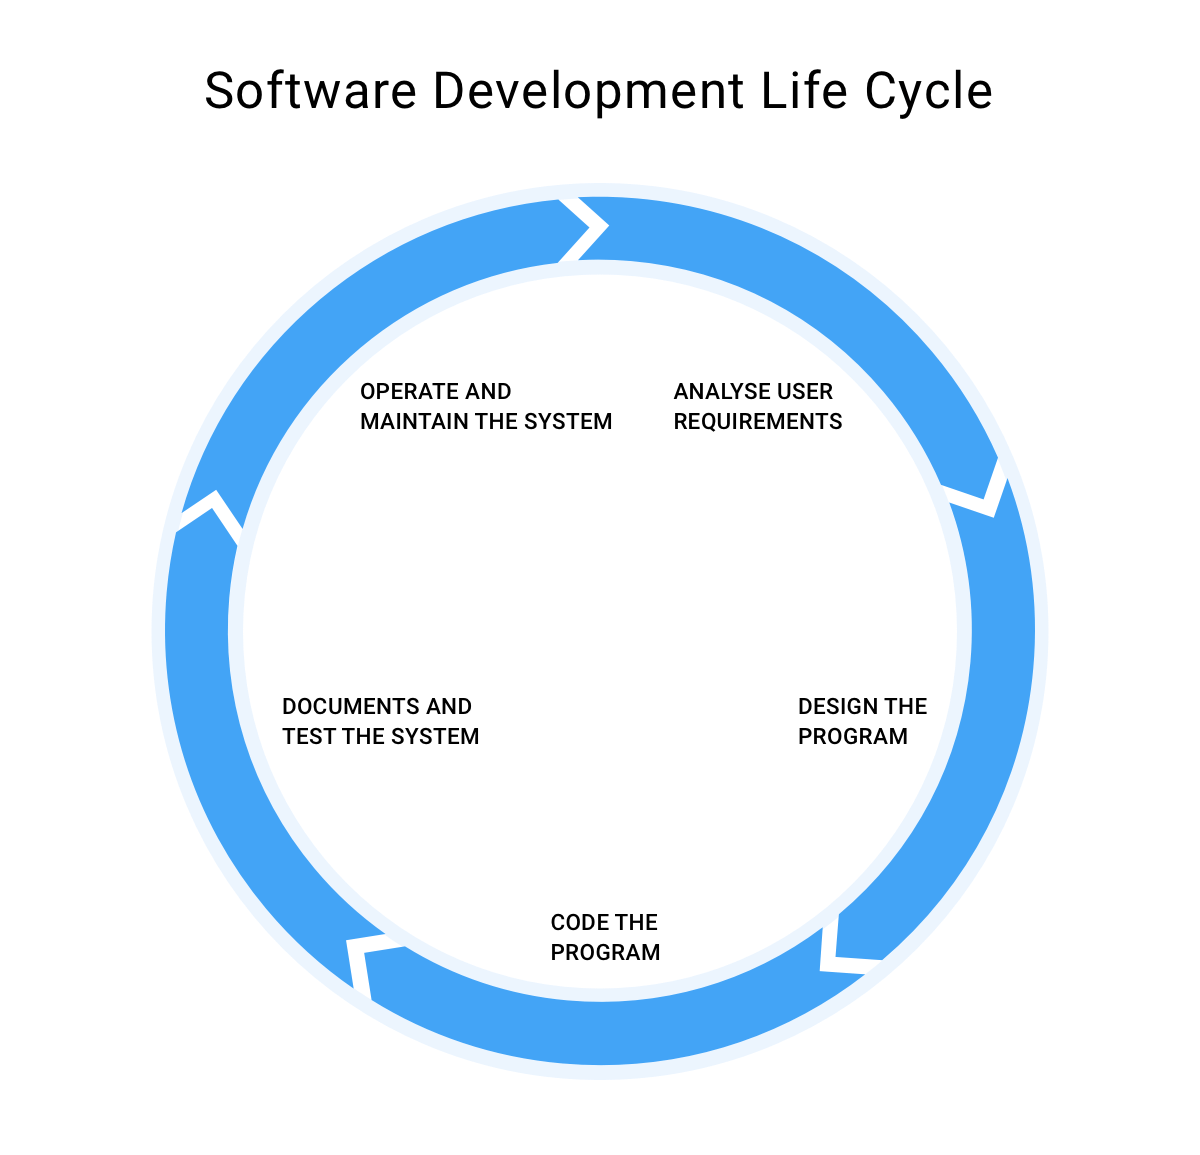
\includegraphics[width=0.4\linewidth, height=0.7\textheight]{content/img/software-development-cycle}
		\caption{Software Development Cycle}
		\label{fig:software-development-cycle}
	\end{figure}
	
}

\frame{
	\frametitle{SAST vs. DAST}
	\framesubtitle{When to use - Software Development Cycle}
	
	\begin{figure}
		\centering
		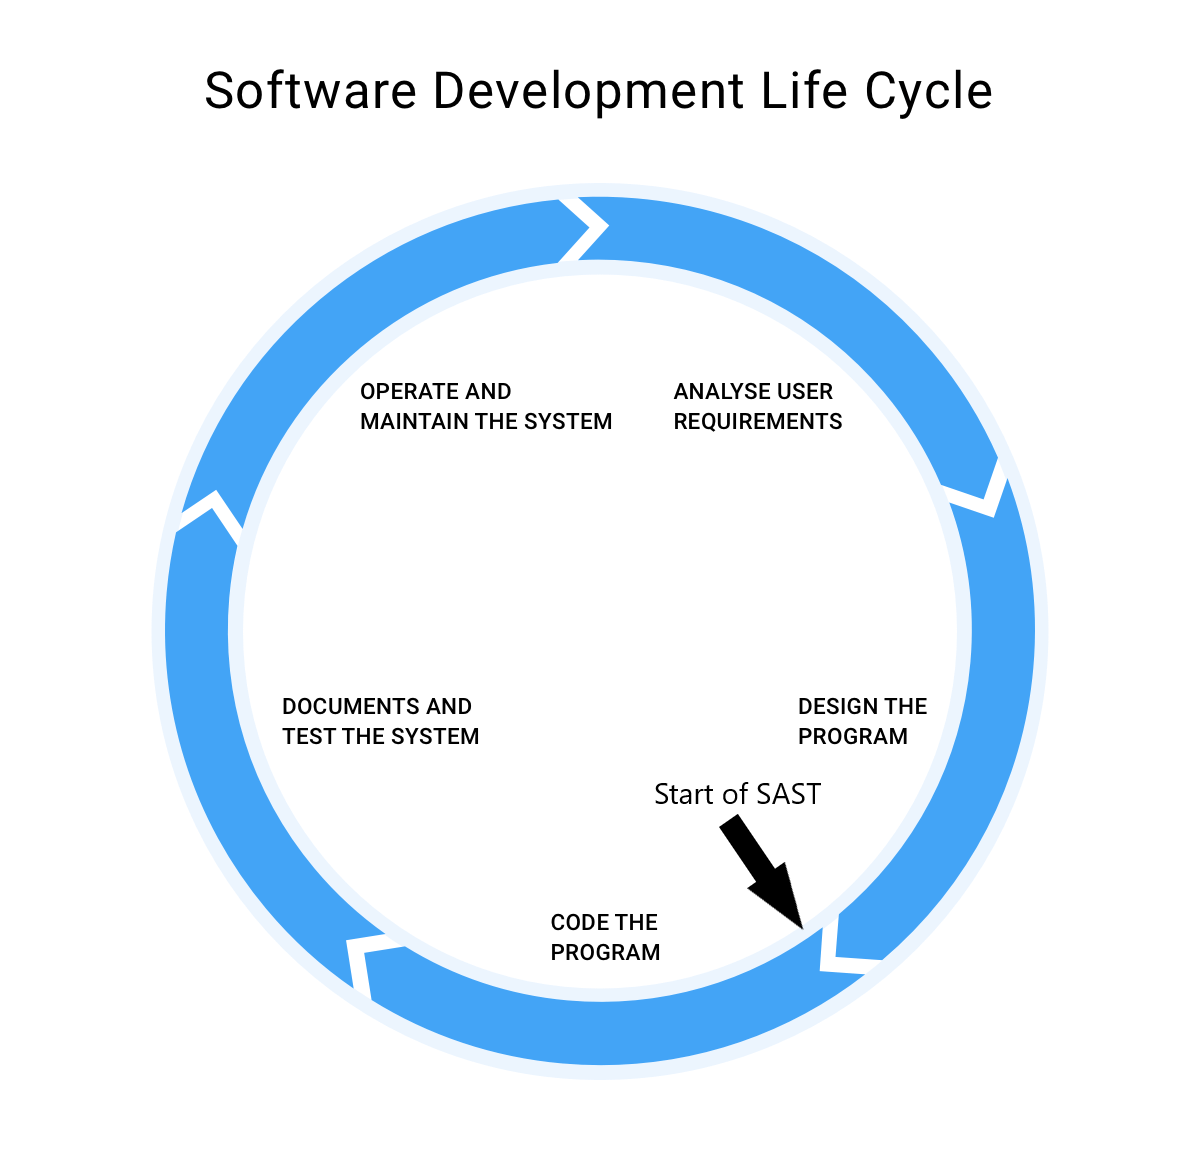
\includegraphics[width=0.4\linewidth, height=0.7\textheight]{content/img/software-development-cycle-sast}
		\caption{Software Development Cycle}
		\label{fig:software-development-cycle}
	\end{figure}
	
}

\frame{
	\frametitle{SAST vs. DAST}
	\framesubtitle{When to use - Software Development Cycle}
	
	\begin{figure}
		\centering
		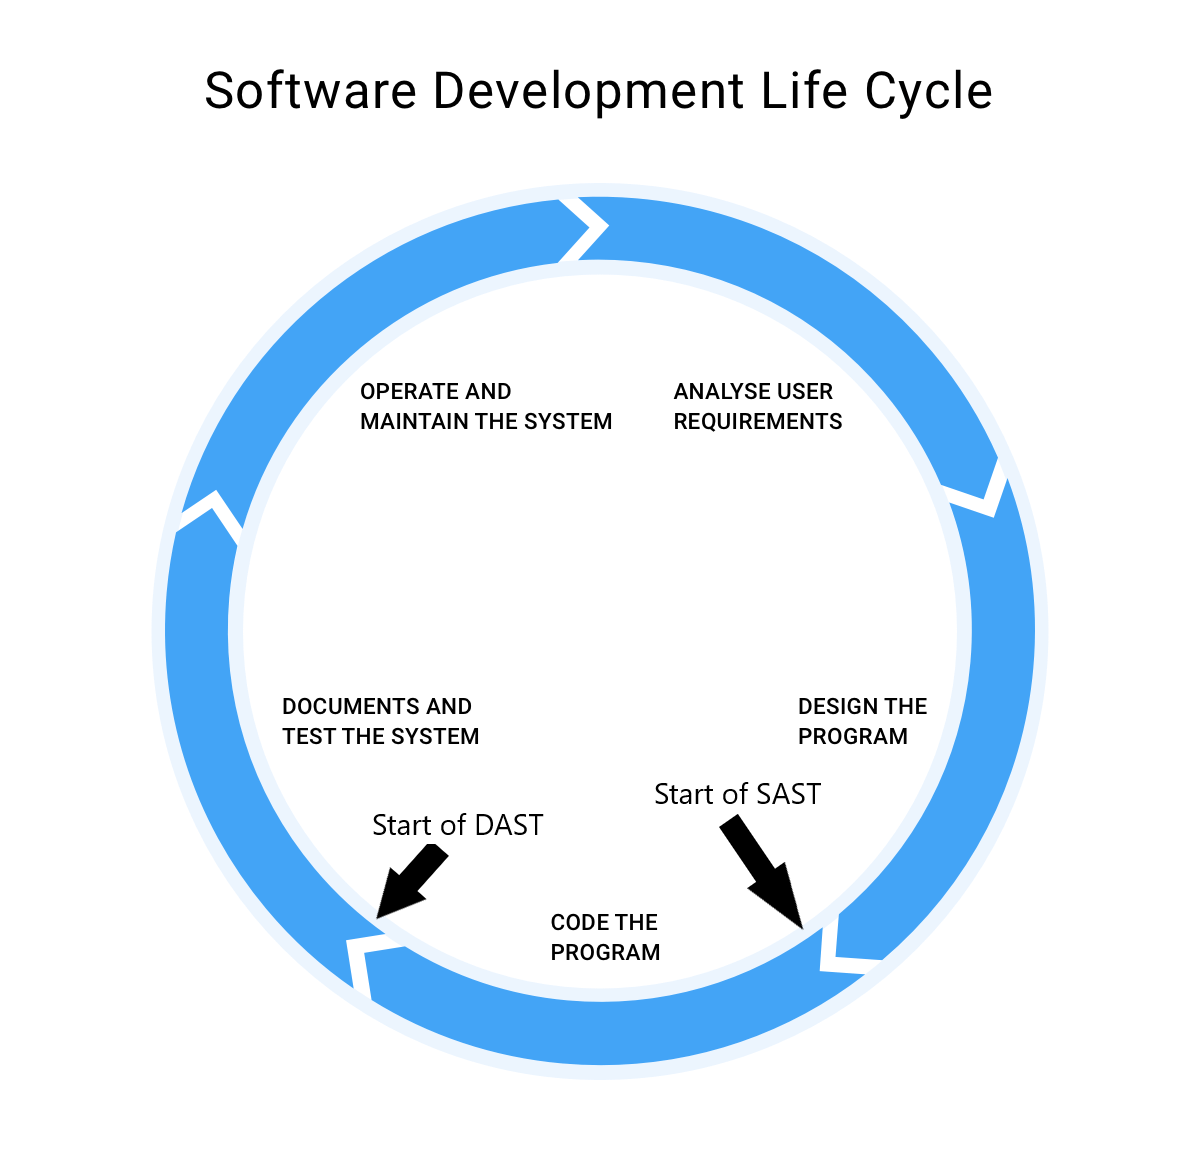
\includegraphics[width=0.4\linewidth, height=0.7\textheight]{content/img/software-development-cycle-sast-dast}
		\caption{Software Development Cycle}
		\label{fig:software-development-cycle}
	\end{figure}
	
}

\frame{
	\frametitle{SAST vs. DAST}
	\framesubtitle{SAST - Vulnerabilities}
	
	\begin{itemize}
		\item Buffer overflows
		\item SQL injection flaws
	\end{itemize}
}

\frame{
	\frametitle{SAST vs. DAST}
	\framesubtitle{DAST - Vulnerabilities}
	
	\begin{itemize}
		\item XSS
		\item SQL injections
	\end{itemize}
}